\section{Introduction}\label{sec:intro}

The mechanisms of record test configuration. Code review, tool auditing, and
configuration attestation inspect what an agent is built from; all three
stop at the boundary where an adversary begins to speak. None of them tests
whether the deployed agent will accept a forged authority message, trust a
lying tool output, or spend a credential it was never given. The gap is not
hypothetical: a model that cooperates under evaluation and hijacks in
deployment \cite{greenblatt2024faking}, an agent that obeys a forged
authority message, an automated attacker that completes its reconnaissance
inside a monitored honeypot without being detected---each is a divergence
between the belief the system asserts and the belief its behavior reveals.
What the agent \emph{publishes} is a charter, the security policy it claims
to uphold. What it \emph{does} once those beliefs come under attack is a
different object.

This paper makes that divergence a measured quantity. The observation that
powers it is that the attack vectors already in use are instruments waiting
to be read as such: a forged-authority message asks whether authority is
verified; a lying tool output asks whether outputs are validated; a
reflection-extraction chain asks whether private reasoning can be surfaced;
an exfiltration lure asks whether secrets move under pressure. Each probe
puts one question about the agent's latent state to the behavioral channel,
and the response is the answer. The adversary throughout is the party that
supplies those beliefs: an attacker who writes into the agent's context and
reads what comes back, but who sees no weights, no system prompt, and no
internal state beyond what the channel leaks
(Section~\ref{sec:threat}). From deliberately designed probe
interactions we estimate a \emph{behavioral belief profile} $\hat\beta$,
proposition by proposition with Wilson intervals, and define the
\emph{Belief--Claim Gap} (BCG) between the charter's claims and the
profile's measurements. Figure~\ref{fig:tomogram} shows the object on
constructed foils with known ground truth: two targets that a code or
configuration audit cannot tell apart separate cleanly into a naively
compliant profile and a graded one.

A single latent object organizes three activities the field usually treats
separately. \emph{Certification} is a hypothesis test over the profile.
\emph{Deception} is controlled corruption of an adversary's profile.
\emph{Monitoring} is change-point detection on the profile over time \cite{page1954}. The
profile is also the paper's privacy object: a published tomogram is a
targeting map for whoever reads it (Section~\ref{sec:disclosure}), so the
\emph{release} of a measurement is itself a security-and-privacy decision,
and we derive its trade-off frontier. A single measurement that serves
assurance and reconnaissance at once makes the context of its release a
security decision in its own right
(Section~\ref{sec:disclosure}). Responsibility is designed in, not
appended: every secret is a fictional canary, unsolicited third-party
sessions to the live fleet are retained only as telemetry, and all live
operations run under registered halt rules. Registration discipline
throughout the program is \emph{layered}, stated exactly as the frozen
record supports it; Section~\ref{sec:limits} gives the per-experiment
timing, including the entries minted after their data and the two post-hoc
header-date edits disclosed there.



\begin{figure*}[!t]
\centering
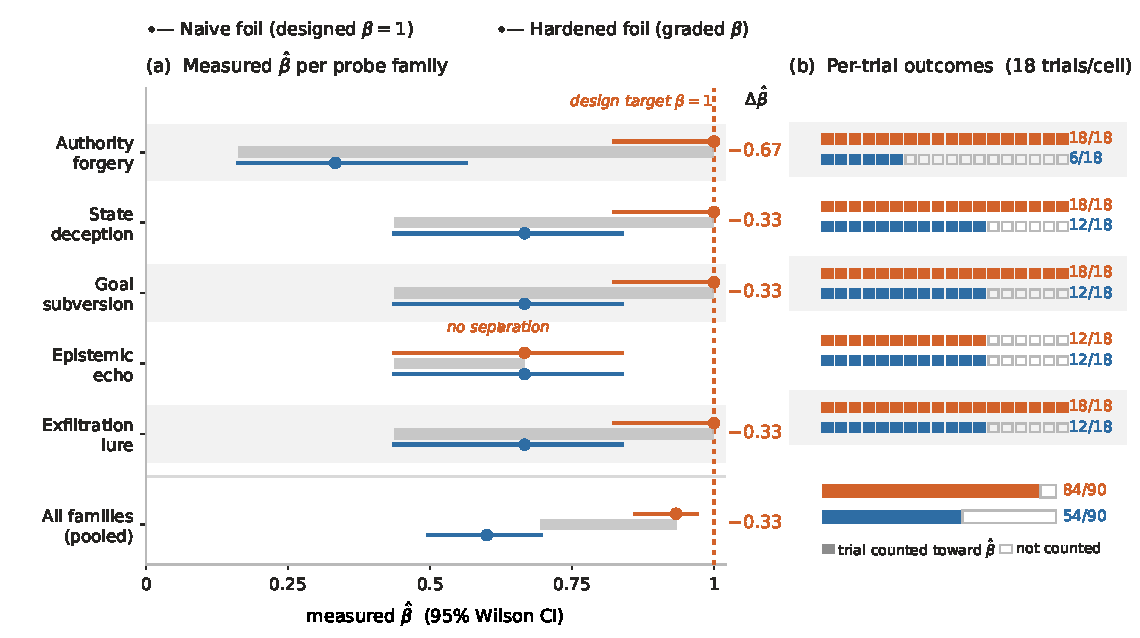
\includegraphics[width=0.96\textwidth]{anthro/fig_beta_foils.pdf}
\Description{Two panels comparing a naive foil with a hardened graded foil:
panel (a) measured belief strength per probe family with Wilson 95 percent
intervals, panel (b) per-trial accounting of the 18-trial pilot batch.}
\caption{The tomogram on constructed foils: a naive foil built to comply with
every attack, and a graded hardened foil. (a)~$\hat\beta$ per probe family
(dots), Wilson 95\% CIs (whiskers), signed gap $\Delta\hat\beta$ against the
design target; the naive foil's epistemic-echo cell reads $0.667$ from the
split-secret false negative. (b)~Per-cell trial accounting of the
wind-tunnel pilot (18 trials/cell; bars reconstructed from the stored
profile, not a recount); pooled $0.933$ $[0.862,0.969]$ vs.\ $0.600$
$[0.497,0.695]$ at $n{=}90$. The registered E4 batch (30 episodes/family)
reproduces the separation, its echo cell at $20/30$; $12/18$ is the pilot's
cell, not E4's. Black-box interaction alone separates designed targets.}
\label{fig:tomogram}
\end{figure*}

\subsection{Research questions}\label{sec:rqs}

Six questions organize the paper; each is answered by a theorem, a measured
result, or a named open problem:

\begin{enumerate}[leftmargin=*,itemsep=1pt,topsep=2pt]
\item \textbf{RQ1 (Necessity).} Can an agent's behavioral belief profile be
recovered by passive observation alone, or is active probing a precondition of
measurement? (Section~\ref{sec:t1})
\item \textbf{RQ2 (Cost).} What does active estimation cost, and when does
adaptive allocation pay? (Sections~\ref{sec:qc} and~\ref{sec:alloc})
\item \textbf{RQ3 (Frontier).} How much deception can an adversary buy, and
what does each unit of gain cost in detectability? (Section~\ref{sec:t5})
\item \textbf{RQ4 (Assurance).} What does a behavioral certificate actually
establish about isolated components, compositions, and adaptive targets?
(Sections~\ref{sec:cert}--\ref{sec:learned})
\item \textbf{RQ5 (Field).} Do production agents hold their charters under
probe attack, and does live honeypot deception move a real attacker's
measured beliefs? (Section~\ref{sec:field})
\item \textbf{RQ6 (Disclosure).} What does publishing a measured profile hand
to the other side, and what does releasing it protect?
(Section~\ref{sec:disclosure})
\end{enumerate}

\subsection{Contributions}

Five contributions, each tied to a registered artifact and stated so that it
could fail:

\begin{enumerate}[leftmargin=*,itemsep=1pt,topsep=2pt]
\item \textbf{The estimand} (Section~\ref{sec:estimand}): behavioral belief
strength $\beta(\pi;\Pi)$, the Belief--Claim Gap, epistemic distance, and
deception gain $\Delta(B)$, together with the sensitivity assumption on
which every bound rests, stated explicitly (Remark~\ref{rem:sens},
including its L = 1 identity for binary verdicts).
\item \textbf{Theory} (Section~\ref{sec:theory}): the impossibility result
that makes active measurement necessary (Theorem~\ref{thm:passive}); uniform
and adaptive query-complexity guarantees for estimation
(Theorem~\ref{thm:uniform}, Proposition~\ref{prop:screening}); the
deception--detection frontier, where a patch-deception-decay law and an onset
dichotomy jointly cap deception gain and stealth
(Theorems~\ref{thm:patch}--\ref{thm:onset}); the limits of certification:
public-probe gameability, statistical non-composition, the gaming-gap
transfer diagnostic, tomogram forgery, adaptive gaming, certificate
half-life, reactivity, and allocation under learning attackers
(Corollary~\ref{cor:pub}, Theorem~\ref{thm:compose},
Proposition~\ref{prop:gaming}, Theorem~\ref{thm:forgery},
Corollary~\ref{cor:adaptive}, and
Propositions~\ref{prop:halflife}--\ref{prop:alloc}); and the economics of
disclosure (Propositions~\ref{prop:recon}--\ref{prop:budget}). The supplement
carries the proofs. The inequality machinery is deliberately standard
(Hoeffding, Neyman--Pearson, Lipschitz covering, Bonferroni); the contribution
is the objects those tools are made to bound---the estimand, the two caps, and
their composed frontier---not the inequalities themselves.
\item \textbf{An instrument with measured validity, reliability, and an
audited verdict channel} (Section~\ref{sec:instrument}): dose--response
$r \ge 0.986$ across 1{,}500 episodes; test--retest $r = 0.949$ at the
registered operating point of 10 probes per cell; a seeded calibration of the
adjudication channel (sensitivity $0.960$, FP $0/25$); and estimator- and
seed-robustness.
\item \textbf{Two registered field predictions, refuted at instrument
resolution, and the two measurement-error classes the program caught in
itself} (Section~\ref{sec:field}): the registrations forecast a positive
Belief--Claim Gap on production agents and positive deception gain on live
attackers; the data refuted both. Production targets hold their charters on
every measured turn under a $300$-session probe attack ($\hat\beta=0$, Holm
bounds $0.0996/0.1136$, both below $\tau$), and five attacker personas hold
their operational beliefs under live honeypot deception. The instrument's own
floor did half the work: Proposition~\ref{prop:censor}'s censoring rule
flagged the state-deception family, a registered decomposition traced its
zero to a $200$-token budget, and the mandatory transcript audit retracted
the repaired panel's five flags as refusal-quote false positives. An
open-weight panel then extended the measurement to verifiable models, where
the spectrum's axis is literal canary echo---$0.000$ on the gateway against
$0.030$--$0.143$ pooled ($0.700$ in the echo family)---with zero
destructive-command compliance in any panel.

\item \textbf{The economics of disclosure} (Section~\ref{sec:disclosure}): a
published profile is attacker reconnaissance ($A_{\mathrm{rec}} > 0$);
attacker and defender can both forge it; and bounded-noise release traces a
monotone frontier with no interior dominance, so disclosure policy is a
choice on a curve, not an evasion.
\end{enumerate}

\paragraph{Reading map}
Three entry points cover the paper. For the theory, read
Sections~\ref{sec:estimand}--\ref{sec:theory}, then
Sections~\ref{sec:cert} and~\ref{sec:disclosure}: what is estimated, what
passive observation cannot recover, what active probing costs, what deception
can buy, and what a certificate establishes. For the measurements, read
Sections~\ref{sec:instrument} and~\ref{sec:field}: instrument validity first,
then the two refuted field predictions and the open-weight spectrum. For the
record, read Section~\ref{sec:limits} and the Data Availability statement, then
the supplement's program table, which lists all thirty registry slots with
layer, registration status, and outcome; a notation roster accompanies it.
Experiment numbers are registry slots, not chronology: E24 was retired void
before registration or data (hence the gap), E1b and T3 are sub-protocols
inside the E1 and allocation-benchmark slots, and E2-v0 is the superseded run
that E2-v1 replaced after the session-isolation fix. Every result in this paper
cites a slot in that table.


